\section{Medium Modification and EMC Effect}
  The nucleons in the SRC acquire high momenta through the short distance parts of the NN interaction. While the typical radius of a nucleon is roughly 0.85 fm~\cite{xiaohui}, the strong repulsive core in the NN interaction appears below 1 fm, which means that the wave-functions of these nucleons have significant overlap. One may argue that the structures and properties of these nucleons at close distance could have been modified in such localized high density configurations. This is generally referred to as medium modification~\cite{john_src_emc}. The inter-nucleon separation in heavy nuclei is typically smaller than the one in light nuclei, so the medium modification is expected to show a dependence on the average nuclear density.
  
 In Eq.~\eqref{src_a2}, the magnitude of the SRC in $1.3\leq x_{bj}<2.0$ is given by the scale factor, $\mathrm{a_{2}}$, which only depends on the nuclear number A in this region. Studies of the A-dependence of the SRC have been recently performed in Ref.~\cite{PhysRevLett.106.052301, john_src_emc} by combining the results of measurements in SLAC~\cite{SLAC_Measurement_PRC.48.2451}, Hall-B~\cite{PhysRevLett.96.082501} and JLab Hall-C~\cite{PhysRevLett.108.092502}. A different quantity, $\mathrm{R_{2N}}$, which is derived from $\mathrm{a_{2}}$ and includes a center of mass (c.m.) motion correction, is more applicable for this kind of study. While $\mathrm{a_{2}}$ represents the relative strength of the high-momentum tail in the nucleus, $\mathrm{R_{2N}}$ refers to the probability of a nucleon being part of a SRC configuration in a nucleus A compared with a nucleon in a deuteron.
 
  \begin{figure}[!ht]
  \begin{center}
    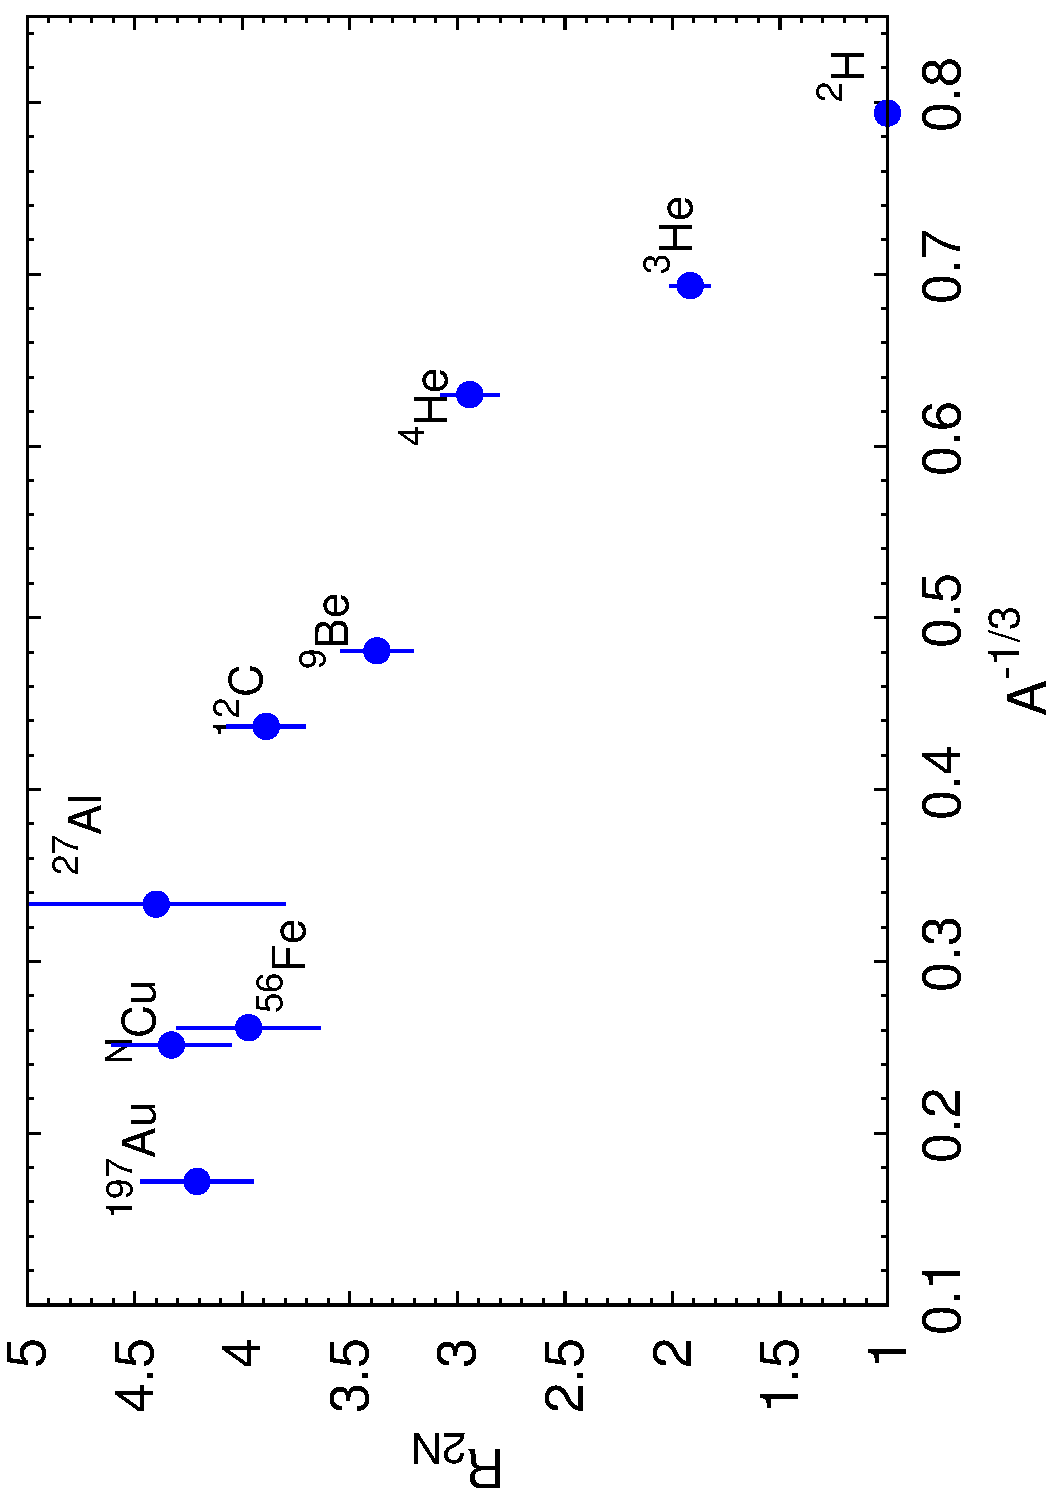
\includegraphics[type=pdf,ext=.pdf,read=.pdf,angle=270,width=0.54\linewidth]{./figures/physics/src_vs_a_third}
    \caption[$\mathrm{R_{2N}}$ vs $\mathrm{A^{-1/3}}$]{\footnotesize{$\mathrm{R_{2N}}$ vs $\mathrm{A^{-1/3}}$ where $\mathrm{R_{2N}}$ in the y-axis is the scaling factor of the 2N-SRC defined in Eq.~\eqref{src_a2} with the center of mass correction. Figure is adopted from Ref.~\cite{john_src_emc}.}}
    \label{src_vs_a}
  \end{center}
\end{figure}  
  \begin{figure}[!ht]
  \begin{center}
    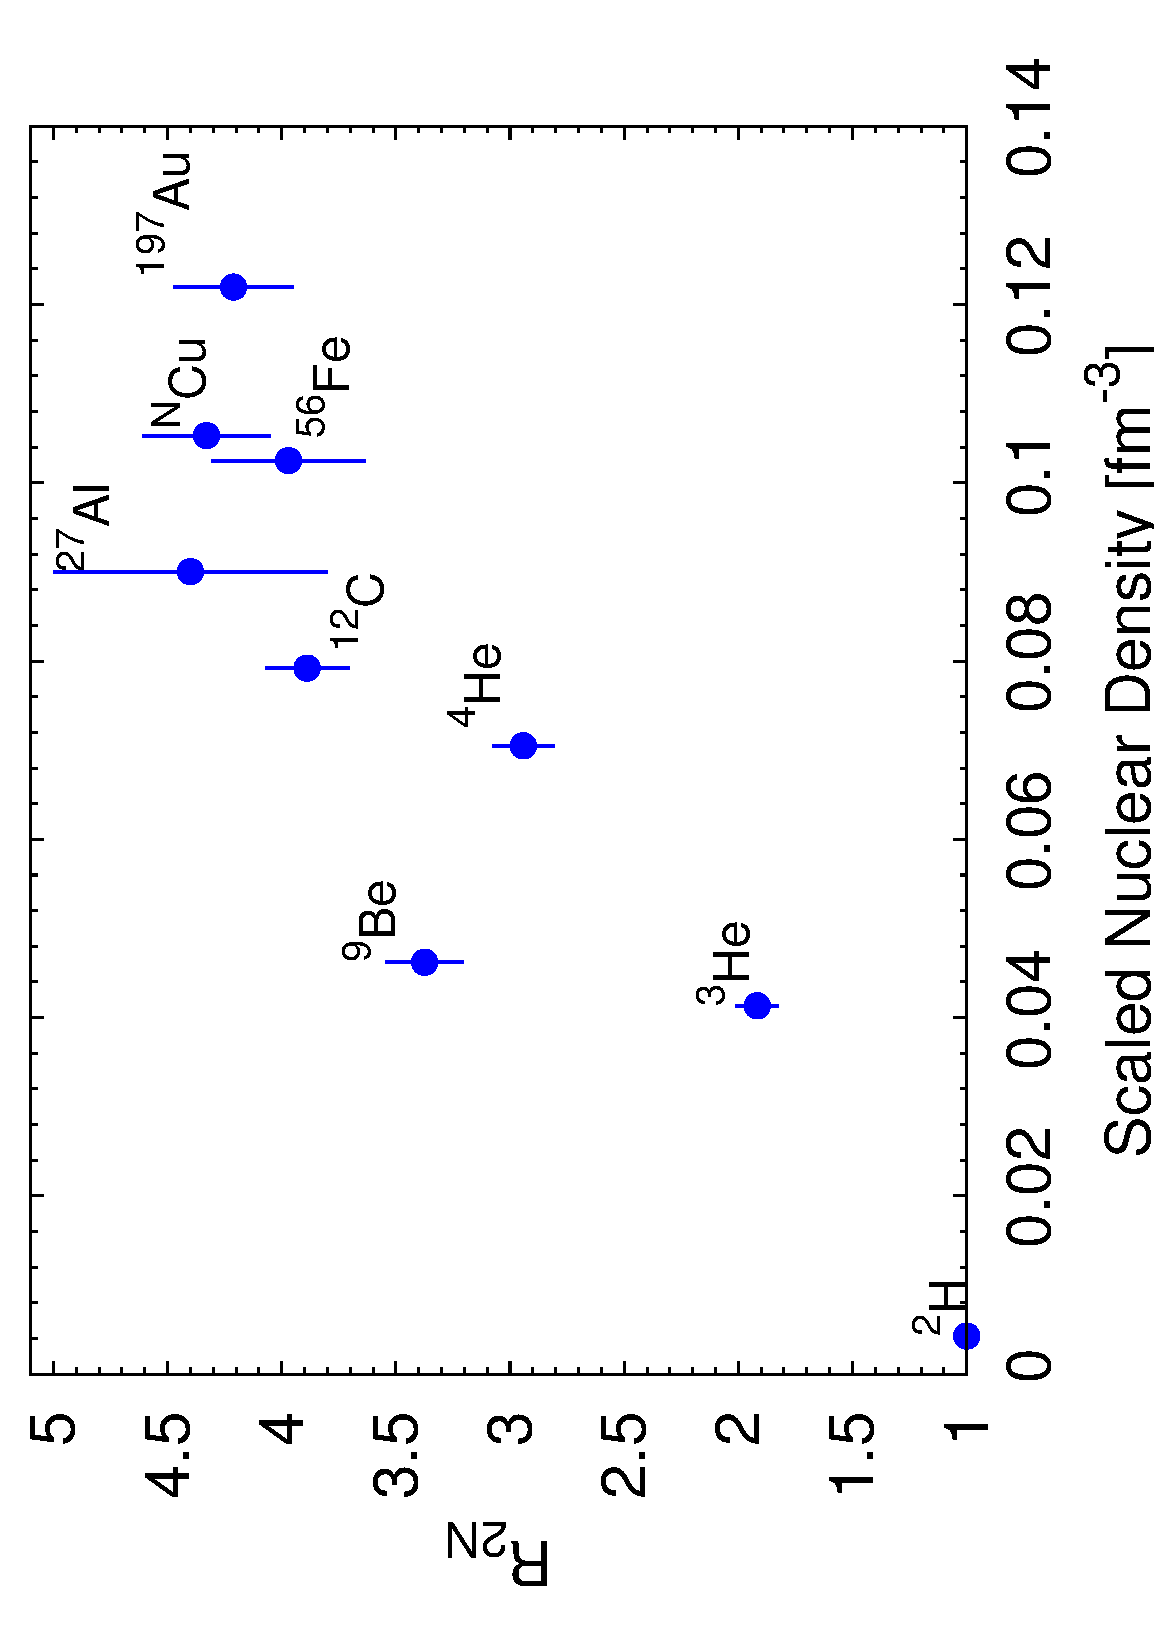
\includegraphics[type=pdf,ext=.pdf,read=.pdf,angle=270,width=0.6\linewidth]{./figures/physics/src_vs_dens_scaled}
    \caption[$\mathrm{R_{2N}}$ vs nuclear density]{\footnotesize{$\mathrm{R_{2N}}$ vs the nuclear density where the scaled nuclear density in x-axis is defined in Eq.~\eqref{density_scaled}. Note that the y-axis is $\mathrm{R_{2N}-1}$. Figure is adopted from Ref.~\cite{john_src_emc}.}}
    \label{src_vs_dens}
  \end{center}
\end{figure}    
  Fig.~\ref{src_vs_a} shows $\mathrm{R_{2N}}$ as a function of $\mathrm{A^{-1/3}}$, which appears to saturate at large A. A linear dependence would be expected if the nuclear response was the incoherent sum of scattering from individual nucleons. In fact, one is more interested in the variation of $\mathrm{R_{2N}}$ in the average nuclear density. A scaled nuclear density is defined as~\cite{john_src_emc}:
  \begin{equation}
    \rho_{scaled}(A) = \frac{A-1}{A}\rho(A),
    \label{density_scaled}
  \end{equation}
where $\rho(A)$ is the actual average nuclear density of the nucleus A, and the correction factor of (A-1)/A accounts for the excess nuclear density seen by the struck nucleon. Fig.~\ref{src_vs_dens} shows $\mathrm{R_{2N}}$ as a function of the scaled nuclear density. The figure indicates a nearly linear correlation for most nuclei except for $\mathrm{^{9}Be}$. 

\begin{figure}[!ht]
  \begin{center}
    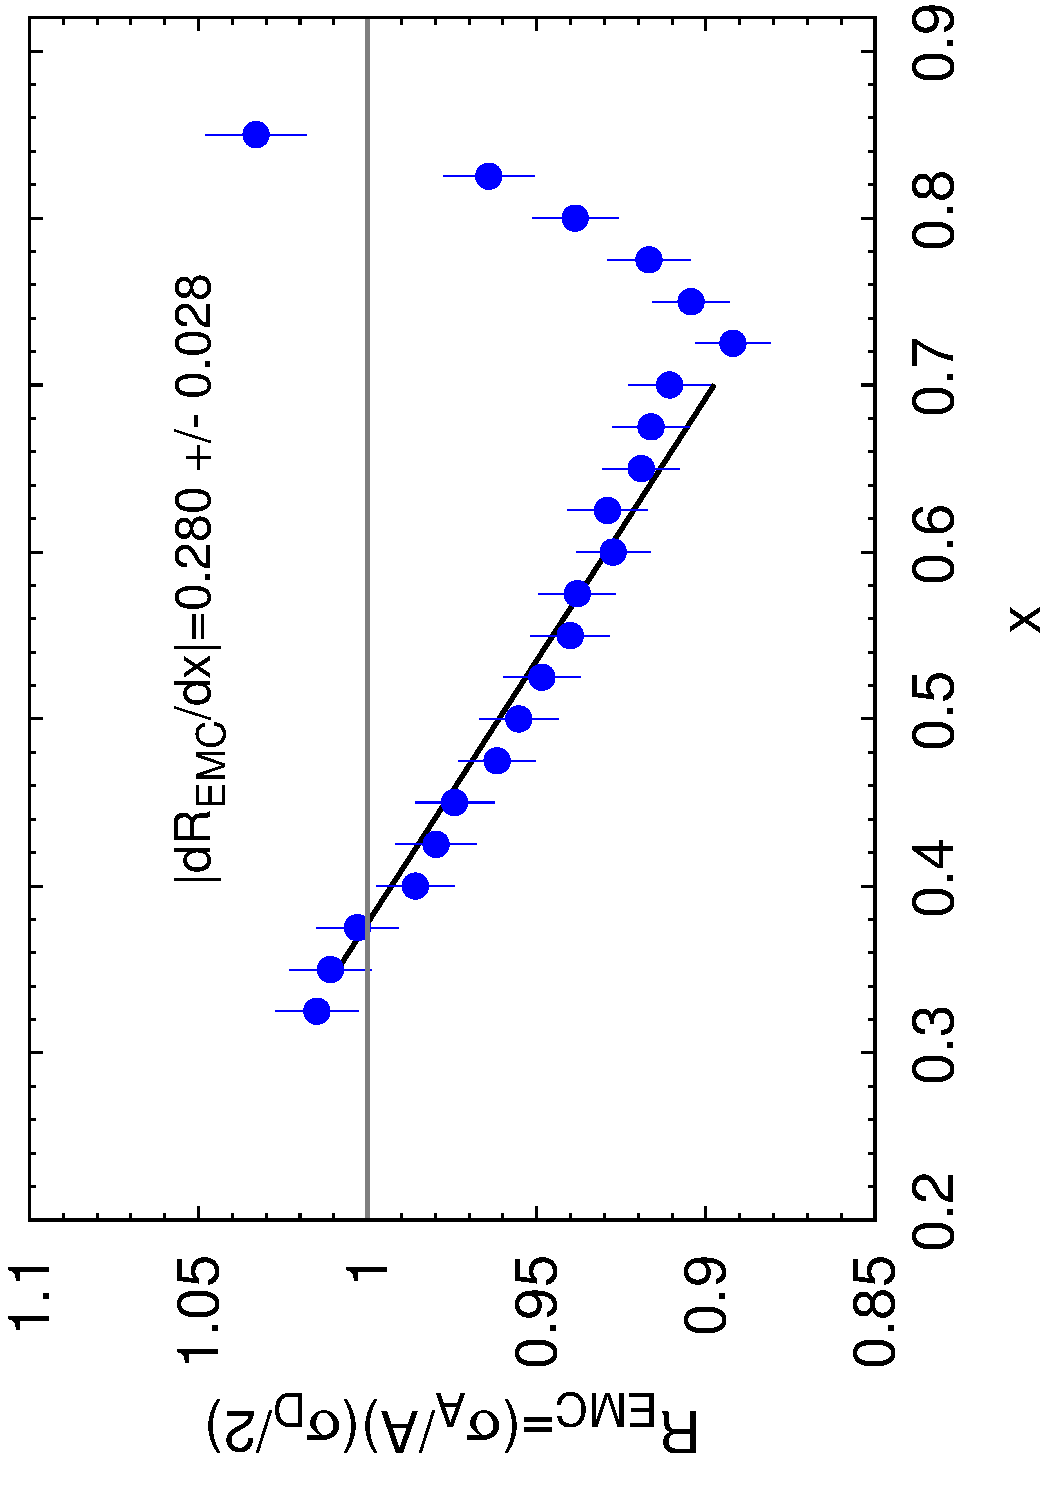
\includegraphics[type=pdf,ext=.pdf,read=.pdf,angle=270,width=0.60\linewidth]{./figures/physics/e03103_carbon}
    \caption[The EMC effect]{\footnotesize{The EMC effect illustrated by the slope of the ratio of the per-nucleon inclusive DIS cross sections of $\mathrm{^{12}C}$ to those of deuteron. Figure is adopted from Ref.~\cite{PhysRevLett.103.202301}.}}
    \label{emc_slop_03013}
  \end{center}
\end{figure}  
 The average density dependence in the SRC shown in Fig.~\ref{src_vs_dens} has also been seen in the analysis of the EMC effect, which refers to the in-medium modification of the nucleon structure, $\mathrm{F_{2}}$~\cite{EMC_Review_1995, EMC_Review_2003}. It was first discovered in the mid 1980s~\cite{EMC_first} and confirmed by many other measurements. In these inclusive DIS measurements, the per-nucleon cross sections (proportional to $\mathrm{F_{2}}$) in nuclei were compared to the deuteron at $\mathrm{Q^{2}\geq 2~GeV^{2}}$ and $0.35\leq x_{bj} \leq 0.7$ and turned out to be smaller. As an example, Fig.~\ref{emc_slop_03013} from Ref.~\cite{PhysRevLett.103.202301} shows an $x_{bj}$-dependence of the ratio of the $\mathrm{^{12}C}$ to deuteron deviates from one and decreases for an increasing $x_{bj}$. Many different models have been proposed to explain the EMC effect~\cite{EMC_Review_1995, EMC_Review_2003}. One common assumption is that the modification of the nucleon structure is driven by the average nuclear density. 
 
 \begin{figure}[!ht]
  \begin{center}
    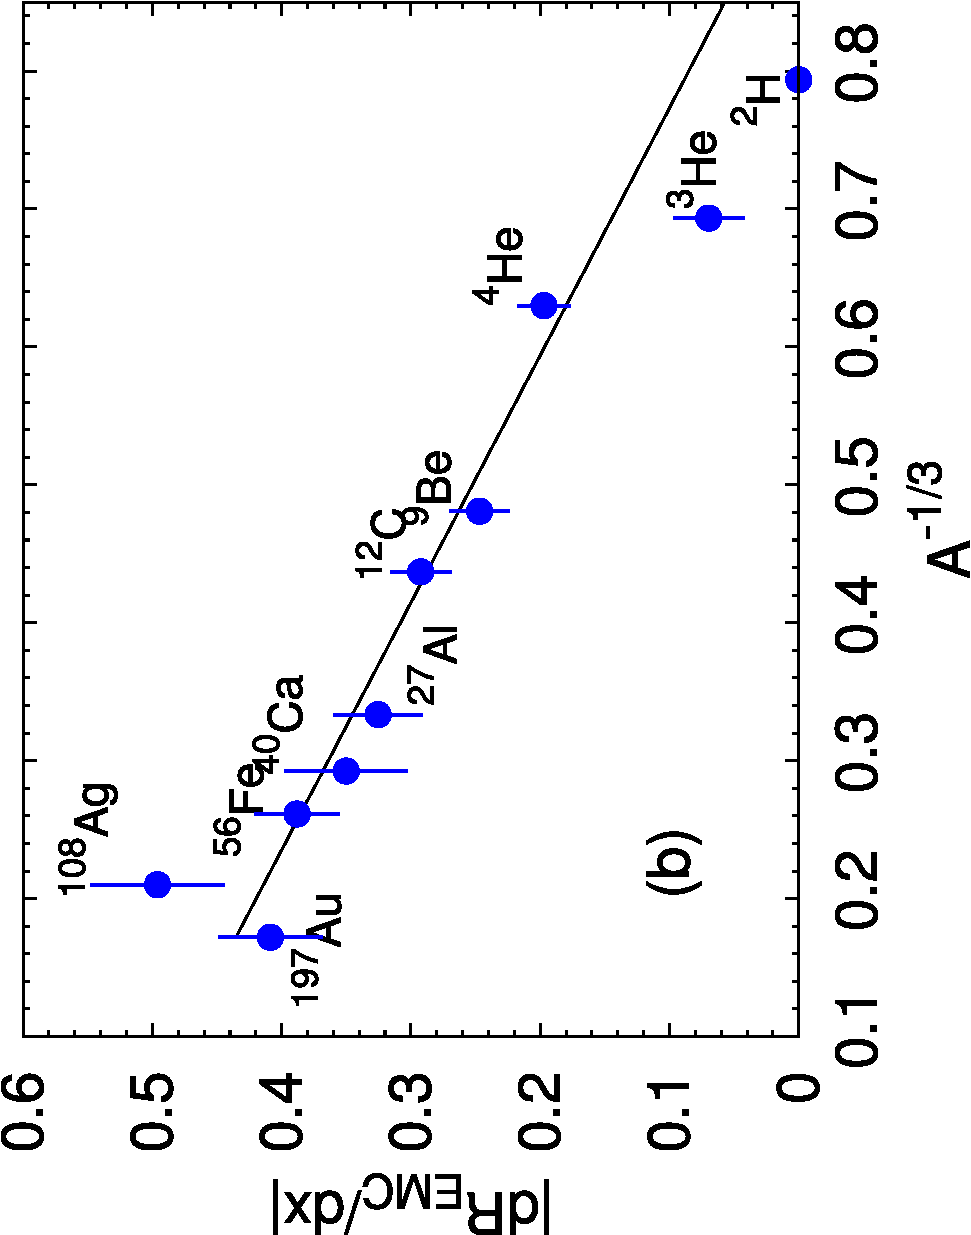
\includegraphics[type=pdf,ext=.pdf,read=.pdf,angle=270,width=0.54\linewidth]{./figures/physics/emc_vs_a_third}
   \caption[$\mathrm{dR_{EMC}/dx}$ vs $\mathrm{A^{-1/3}}$]{\footnotesize{$\mathrm{dR_{EMC}/dx}$ vs $\mathrm{A^{-1/3}}$. Figure is adopted from Ref.~\cite{john_src_emc}.}}
    \label{emc_vs_a}
  \end{center}
\end{figure}   
  The magnitude of the EMC effect can be characterized by the slope of a linear fit to this region, i.e., $\mathrm{dR_{EMC}/dx}$, shown in Fig.~\ref{emc_slop_03013}. The values of $\mathrm{dR_{EMC}/dx}$ for a wide range of nuclei are correlated with $\mathrm{A^{-1/3}}$, and the result given in Fig.~\ref{emc_vs_a} does indicate a linear connection. This result would be expected if the "surface" density distribution is independent of A. However, for light nuclei ($A\leq 12$), this assumption is invalid~\cite{john_src_emc}, so this simple A-dependence study of the EMC effect may be inappropriate. 

   \begin{figure}[!ht]
  \begin{center}
    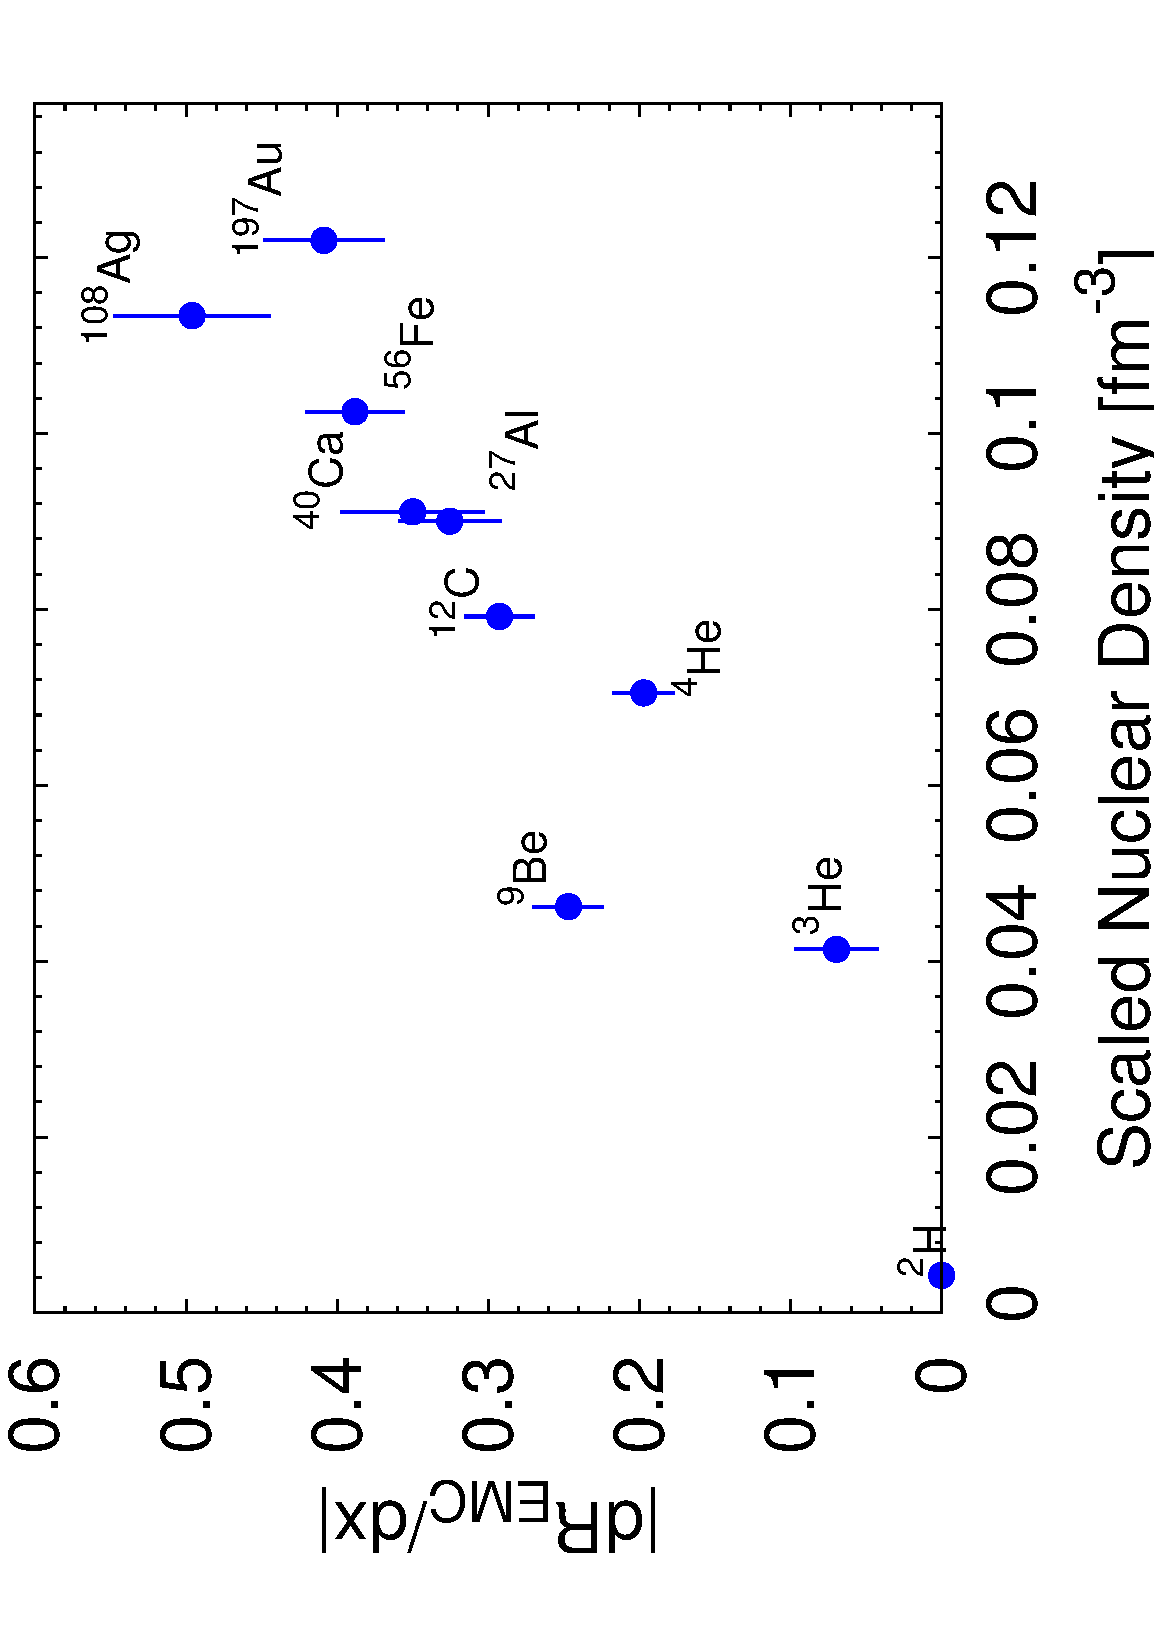
\includegraphics[type=pdf,ext=.pdf,read=.pdf,angle=270,width=0.6\linewidth]{./figures/physics/emc_vs_dens_scaled}
   \caption[$\mathrm{dR_{EMC}/dx}$ vs nuclear density]{\footnotesize{$\mathrm{dR_{EMC}/dx}$ vs the nuclear density where in x-axis the scaled nuclear density defined in Eq.~\eqref{density_scaled}. Figure is adopted from Ref.~\cite{john_src_emc}.}}
    \label{emc_vs_dens}
  \end{center}
\end{figure} 
   The plot of $\mathrm{dR_{EMC}/dx}$ as a function of the scaled average nuclear density in Fig.~\ref{emc_vs_dens} also presents a linear correlation for most nuclei, but $\mathrm{^{9}Be}$, similar to the $\mathrm{R_{2N}}$ distribution in Fig.~\ref{src_vs_dens}, significantly deviates from the linear pattern. It was suggested that, since $\mathrm{^{9}Be}$ is composed of two $\alpha$-like clusters surrounded by a neutron, the local density is more appropriate for studying the EMC effect~\cite{PhysRevLett.103.202301}. 

\begin{figure}[!ht]
  \begin{center}
    \subfloat[EMC and SRC vs A]{
      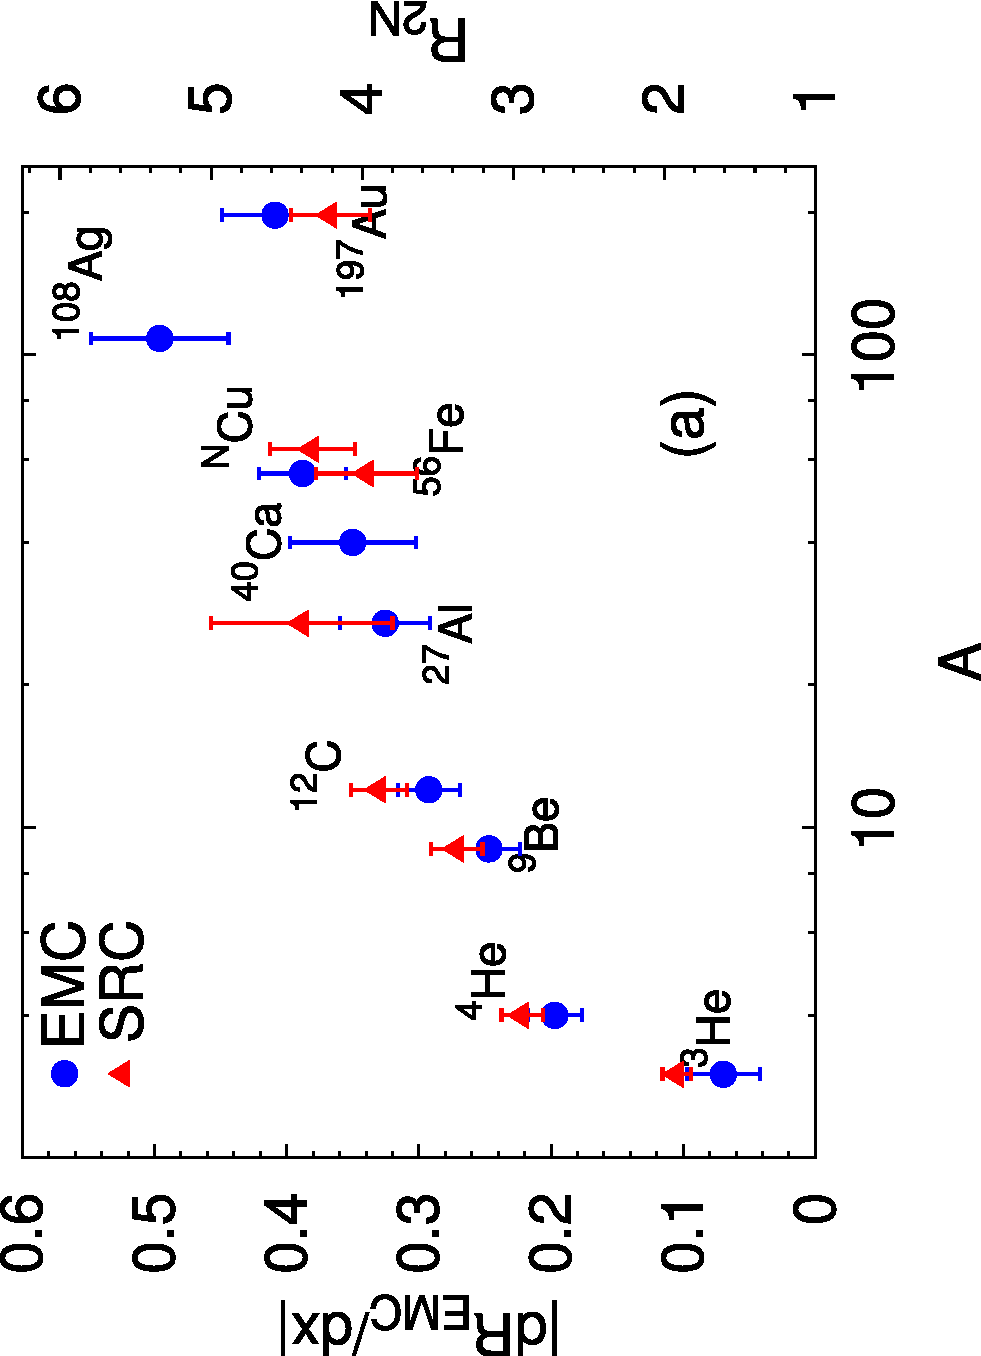
\includegraphics[type=pdf,ext=.pdf,read=.pdf,angle=270,width=0.6\textwidth]{./figures/physics/emc_src_vs_a}
      \label{emc_src_a_all}
    }
    \\ 
    \subfloat[EMC and SRC vs nuclear density]{
      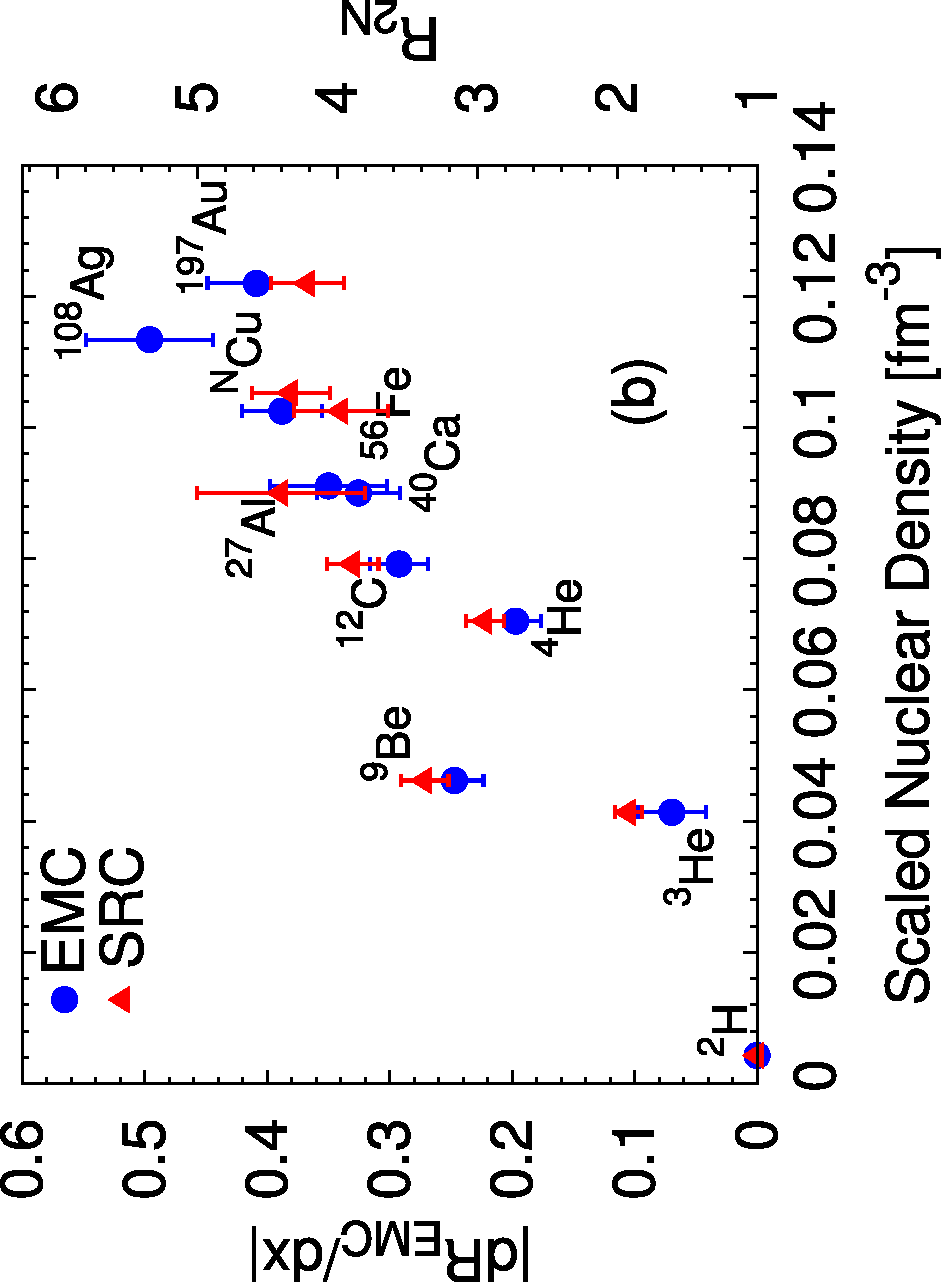
\includegraphics[type=pdf,ext=.pdf,read=.pdf,angle=270,width=0.6\textwidth]{./figures/physics/emc_src_vs_dens}
    \label{emc_src_dens_all}    
    }
    \caption[Connecting EMC and SRC effects]{\footnotesize{Connecting EMC and SRC effects, where $\mathrm{dR_{EMC}/dx}$ and $\mathrm{R_{2N}}$ are shown as a funciton of A (top) and the scaled nuclear density (bottom). Figure is adopted from Ref.~\cite{john_src_emc}.}}
    \label{emc_src_all}
  \end{center}
\end{figure}
  In Fig.~\ref{emc_src_a_all} and Fig.~\ref{emc_src_dens_all}, the A- and density-dependence of $\mathrm{dR_{EMC}/dx}$ and $\mathrm{R_{2N}}$ are directly compared. Remarkably, the same pattern for all nuclei, including $\mathrm{^{9}Be}$, are seen in both plots. Since the measurements of the SRC directly probe the high density configurations inside the nucleus, the results strongly suggest that the local density is driving both of these disparate effects. 
  
    \begin{figure}[!ht]
  \begin{center}
    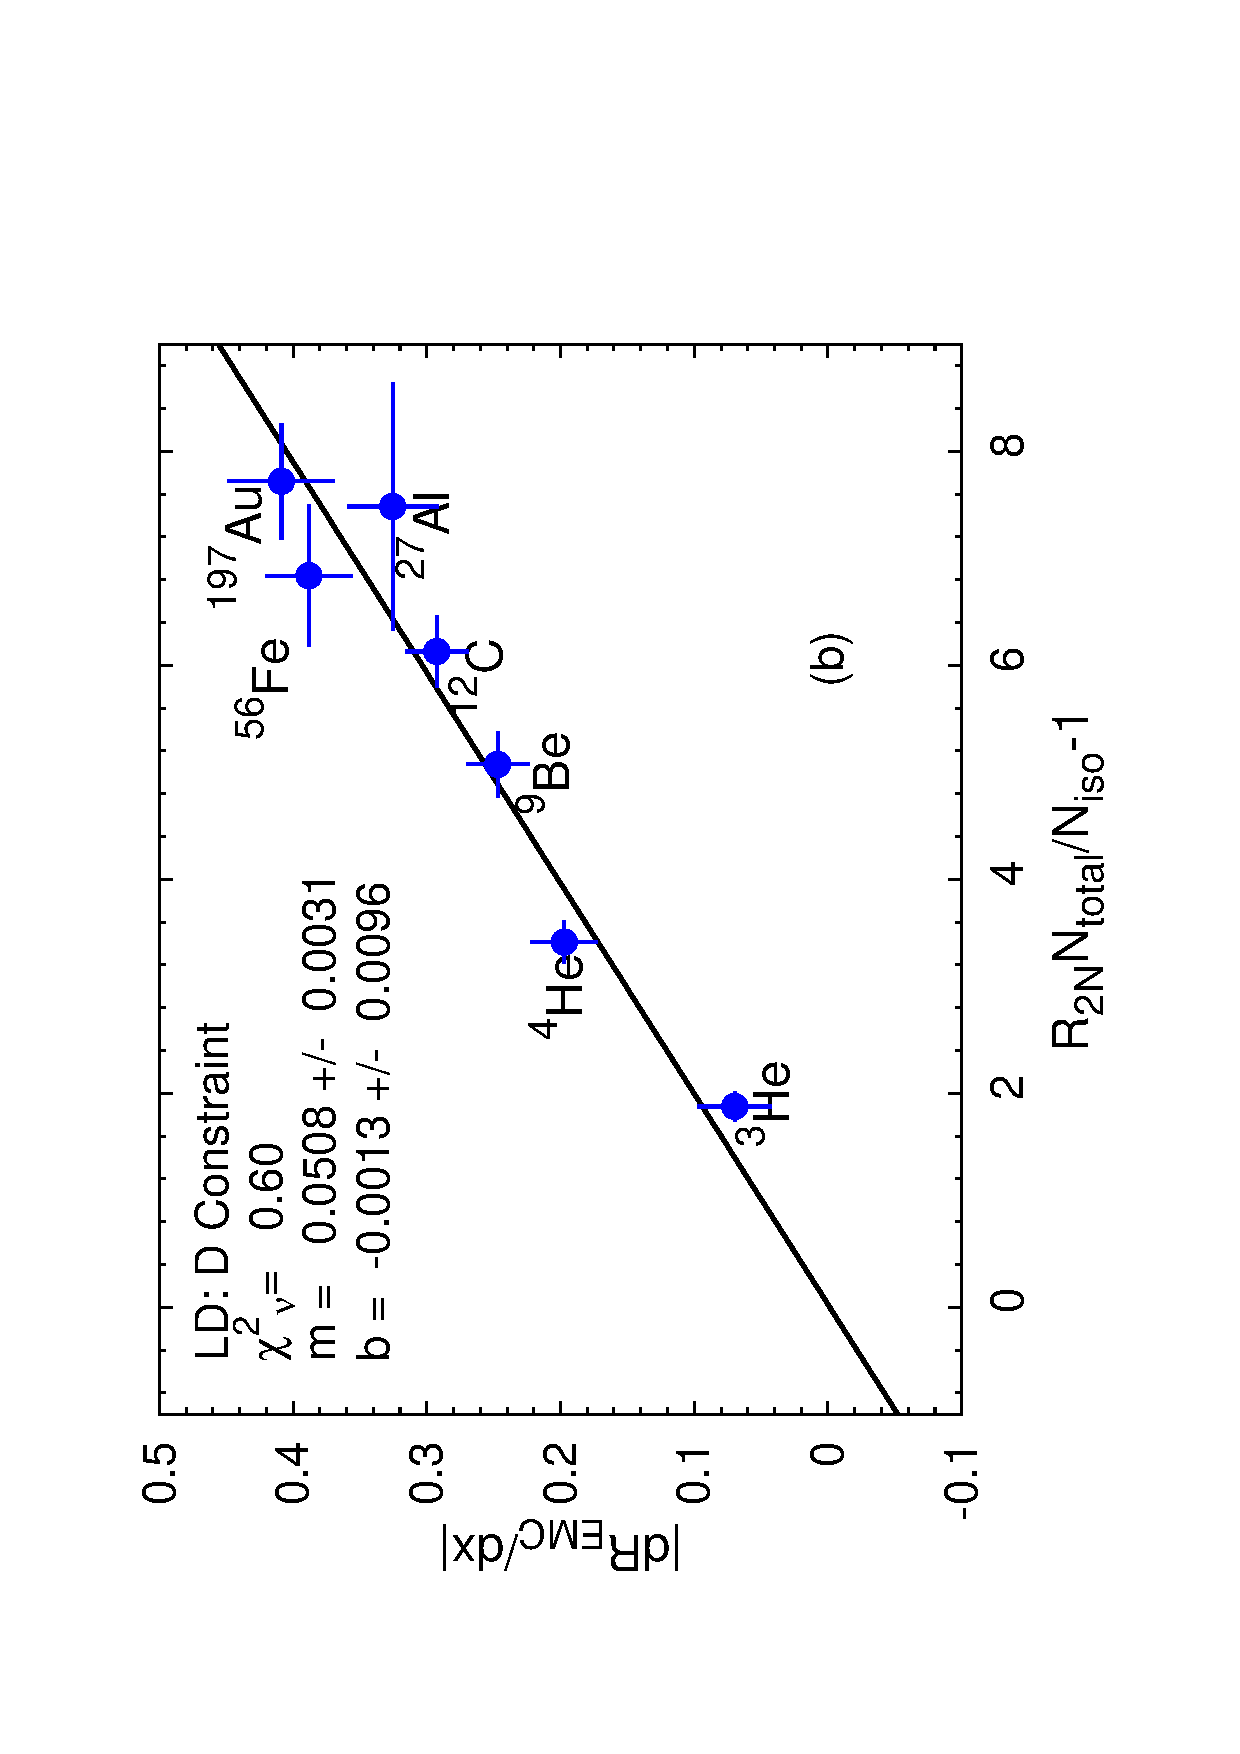
\includegraphics[type=pdf,ext=.pdf,read=.pdf,angle=270,width=0.60\linewidth]{./figures/physics/emc_vs_src_plotfit}
   \caption[$\mathrm{dR_{EMC}/dx}$ vs $\mathrm{R_{2N}}$]{\footnotesize{$\mathrm{dR_{EMC}/dx}$ vs $\mathrm{R_{2N} N_{total}/N_{iso}-1}$, where $N_{total}=A(A-1)/2$ and $N_{iso}=Z(A-Z)$~\cite{john_src_emc}. The plot clearly shows the strong linear correlation between the EMC and the SRC effects. Figure is provided by Ref.~\cite{john_src_emc}.}}
    \label{emc_vs_src}
  \end{center}
\end{figure} 
 The linear connection between the EMC effect and the SRC can be seen in Fig.~\ref{emc_vs_src} where $\mathrm{dR_{EMC}/dx}$ is plotted against $\mathrm{R_{2N}N_{total}/N_{iso}-1}$ with $N_{total}=A(A-1)/2$ and $N_{iso}=Z(A-Z)$. This strong correlation provides a new constraint when modeling these two phenomena. The discussion above clearly demonstrates that the local density configuration plays an essential role in driving both the EMC effect and the SRC. Another hypothesis~\cite{PhysRevLett.106.052301} explains the linear connection between these two effects is due to the high virtuality~\cite{M_Sargsian_JPG_29_2003} of the high momentum nucleon. 
  
 Systematically understanding the connection between the SRC and EMC effects is still desirable, and will be of greatest interest in the 12-GeV era at JLab. Several new experiments have been approved to map out the nuclear dependence of these two effects~\cite{E12_10_103_pr,E12_06_105_pr,E12_10_008_pr,E12_11_107_pr,E12_10_003_pr}.
